\section{Introduction}\label{sec:EinleitAnatomie}
	\begin{sloppypar}
	 \begin{description}
	\item \textsc{Your aims of this section:}\\
	Revision of your cell biology knowledge \\
	MRS GREN and the 7 criteria of life \\
	Anatomic terms to locate a specific part of the body \\
	Functions of the 10 organ systems \\
	% Structure and function of a long bone \\
	% Structure and function of the vertebral column \\
	\end{description}
	\end{sloppypar}
\subsection{Mrs Gren -- living or not?}
	\marginnote{\caution[c][blue][Starr]{ch 4.11 p 70 with a short but worthwile reading on ``\textit{what is life?}''}}
		\Kommentar{ 
		Discussion: mankind, nature; what is life; how can we distinguish between living and non living things?
		
		- do you remember Mrs Gren? \rechts \emph{plant, disk of wood, a mouse, beans dry and sprouting, stone, candle, etc}
		}{}{3cm}{}


\textbf{The seven criteria of life:}

	\vspace{4pt}
	\hspace{-1cm}
	\begin{minipage}[htbp]{0.35\textwidth}
	{\includegraphics[width=1\linewidth]{/share/SB_Unterricht/Biologie/bio00-Intro_dt/mrs-Gren_NEU.jpg}}   \captionof{figure}[Mrs Gren von N. Lieske]{Mrs Gren is certainly alive}  	\label{fig:MrsGren}
	\vspace{2pt}
	\end{minipage}
		\hspace{5mm}
		\begin{minipage}{0.7\textwidth}
		    \renewcommand{\arraystretch}{1.8}
		 	    \begin{tabularx}{10cm}[]{p{5cm} p{5cm}} %
	\toprule
	Englisch & Deutsch  \\\midrule
	 \gapa{\textbf{M}otion \hfill} & \gapa{\textcolor{Plum}{Bewegung} \hfill}\\
	 \gapa{\textbf{R}espiration \hfill} & \gapa{\textcolor{Plum}{(Zell-)Atmung} \hfill}\\
	 \gapa{\textbf{S}ensitivity \hfill} & \gapa{\textcolor{Plum}{Erregbarkeit} \hfill}\\    \\[6pt]
	 \gapa{\textbf{G}rowth \hfill} & \gapa{\textcolor{Plum}{Wachstum} \hfill}\\
	 \gapa{\textbf{R}eproduction\hfill} & \gapa{\textcolor{Plum}{Vermehrung} \hfill}\\
	 \gapa{\textbf{E}exretion \hfill} & \gapa{\textcolor{Plum}{Ausscheidung} \hfill}\\
	 \gapa{\textbf{N}utrition \hfill} & \gapa{\textcolor{Plum}{Ernährung} \hfill}\\
	\bottomrule
	\end{tabularx}%
			    \renewcommand{\arraystretch}{1}
		\end{minipage}	
	


\clearpage
\subsection{Do you still remember cell biology?}
\begin{enumerate}[leftmargin=*]
\item  Human bodies are made of cells and therefore we need to revise our knowledge in this topic. (Re-)read the topics indicated in Starr (9ed) and take your own notes - you may rely on them for your test in human biology.
\end{enumerate}
    \enlargethispage{30pt}
    \begin{addmargin*}[0cm]{-5cm}
	\begin{minipage}[!h][][b]{16cm}
		\bgroup \normalsize
		\setcapmargin*[0cm]{0cm}
			\setlength{\extrarowheight}{0pt}	
		 \captionof{table}[]{repetition: numbers indicate the corresponding chapters in Starr, 9ed. Read these chapters and take your own notes!}
	    \begin{tabularx}{16cm}[]{m{4cm} m{12cm}} %
	\toprule
	Chapter & Your  notes \\ \midrule
	2.4 water and life & \Answer{\begin{itemize} 
		\item water is essential to life due to its property as a solvent
		\item adhesion and cohesion; hydrogen bonds; polarity
		\item high temperature capacity
		 \end{itemize}}{1.75cm} \\ \midrule
	3.2 carbohydrates  &  \Answer{\begin{itemize} 
		\item consist of C, H, O
		\item energy carriers and structural materials
		\item simple (1), short-chained (2-10), complex (>>10) carbohydrates
		\end{itemize}}{1.75cm} \\ \midrule
	3.4 proteins, amino-acids  &  \Answer{\begin{itemize}
		 \item amino acids, chains (primary), coils/sheets (secondary), working 3-D (tertiary), aggregates (quarternary) 
		 \item structural materials and functional proteins
		 \item sequence of AA defines structure; struture defines function
		 \end{itemize}}{1.75cm} \\ \midrule 
	4.1 what is a cell?   &  \Answer{\begin{itemize} 
		\item smallest unit of life
		\item  compartments with specific functions (e.g. mitochondria, nucleus, Golgi Apparatus)
		\item  lipid bilayer around (= plasma membrane); cytoplasma; nucleus in eukayryotes; specific size (limitations through surface-to-volume ratio) 
		\end{itemize}}{1.75cm} \\ \midrule
	4.3 biological membranes   &   \Answer{\begin{itemize} 
		\item double layer of phospho-lipids + proteins:  fluid mosaic
		\item barrier around every cell / organelles
		\item cell communication, adhesion, recognition, transport etc.
		\end{itemize}}{1.75cm} \\ \midrule
	4.7 mitochondria &   \Answer{\begin{itemize} 
		\item production of ATP under aerobic conditions
% 		\item 1 to 4 \micro\metre
		\item double membrane around
		\end{itemize}}{1.5cm} \\ \midrule
	Fig. 4.24 cell organelles and structures  &   \Answer{\begin{itemize} 
		\item functions of the different structures / organelles 
		\item differences of plant- and animal-cells
		\end{itemize}}{1.5cm} \\
	\bottomrule
	\end{tabularx}%
	  \label{tab:Repetitionsthemen}%
				 \vspace{2pt}
		 \egroup
	  \end{minipage}
	\end{addmargin*}

	
	
\clearpage 	 \areaset[0cm]{16cm}{26.5cm} 
\subsection{Anatomical terminology: anatomical planes and relative localisation}\label{ssec:OrientierungKoerper}
 Learn to address anatomical planes and directions at a body like the health professionals! 
 
%  
%  In order address the different parts of a body independently from the way one looks at the body, anatomists developed a system to address the different locations. With this system it doesn't make any difference whether you look at a body from the left, the right or from bottom up or from top down.
% 
% 	\begin{enumerate}[itemsep=1.5em, leftmargin=*]   
% 		\item Learn how to use the different anatomical planes \ref{fig:SchnittEbenen}, \textit{sagital plane, median plane, coronal plane, transverse plane} - use light colours in order to colour these planes! \Kommentar{Farbstifte für Kap. \ref{ssec:OrientierungKoerper}}{}{0cm}{}
% 
% 		\item  Figure \ref{fig:AnatomicalTerms} shows relative anatomical terms used to describe any position at a body. Not shown in the figure are the terms \textsc{anterior} and \textsc{posterior}. Often used synonyms for these terms are \textsc{ventral} and \textsc{dorsal}.
% 		
% 		Match these terms with the arrows shown in \ref{fig:AnatTermsApplication} and colour the arrows. 
% 			
% 		\item \textbf{partner work}: Use self adhesive coloured dots in green and red. Stick a green dot on your partner's body' anywhere you like. Stick a red dot on your partner somewhere else. Use the \emph{anatomical terms} to describe the position of the red dot in relation to the green dot! . Repeat this game using all of the anatomical terms, including the synonyms. Change roles afterwards - your partner will stick dots on your body now.
% 		
% 				\Kommentar{rote und grüne Punkte für Kap. \ref{ssec:OrientierungKoerper}}{}{0cm}{}
% 	\end{enumerate}

\enlargethispage{2cm}
         \vspace{-4pt}
% \begin{addmargin*}[3cm]{0cm}

% \hspace{-1.5cm}
	\begin{center}

	\begin{minipage}[htbp]{12cm}
 		{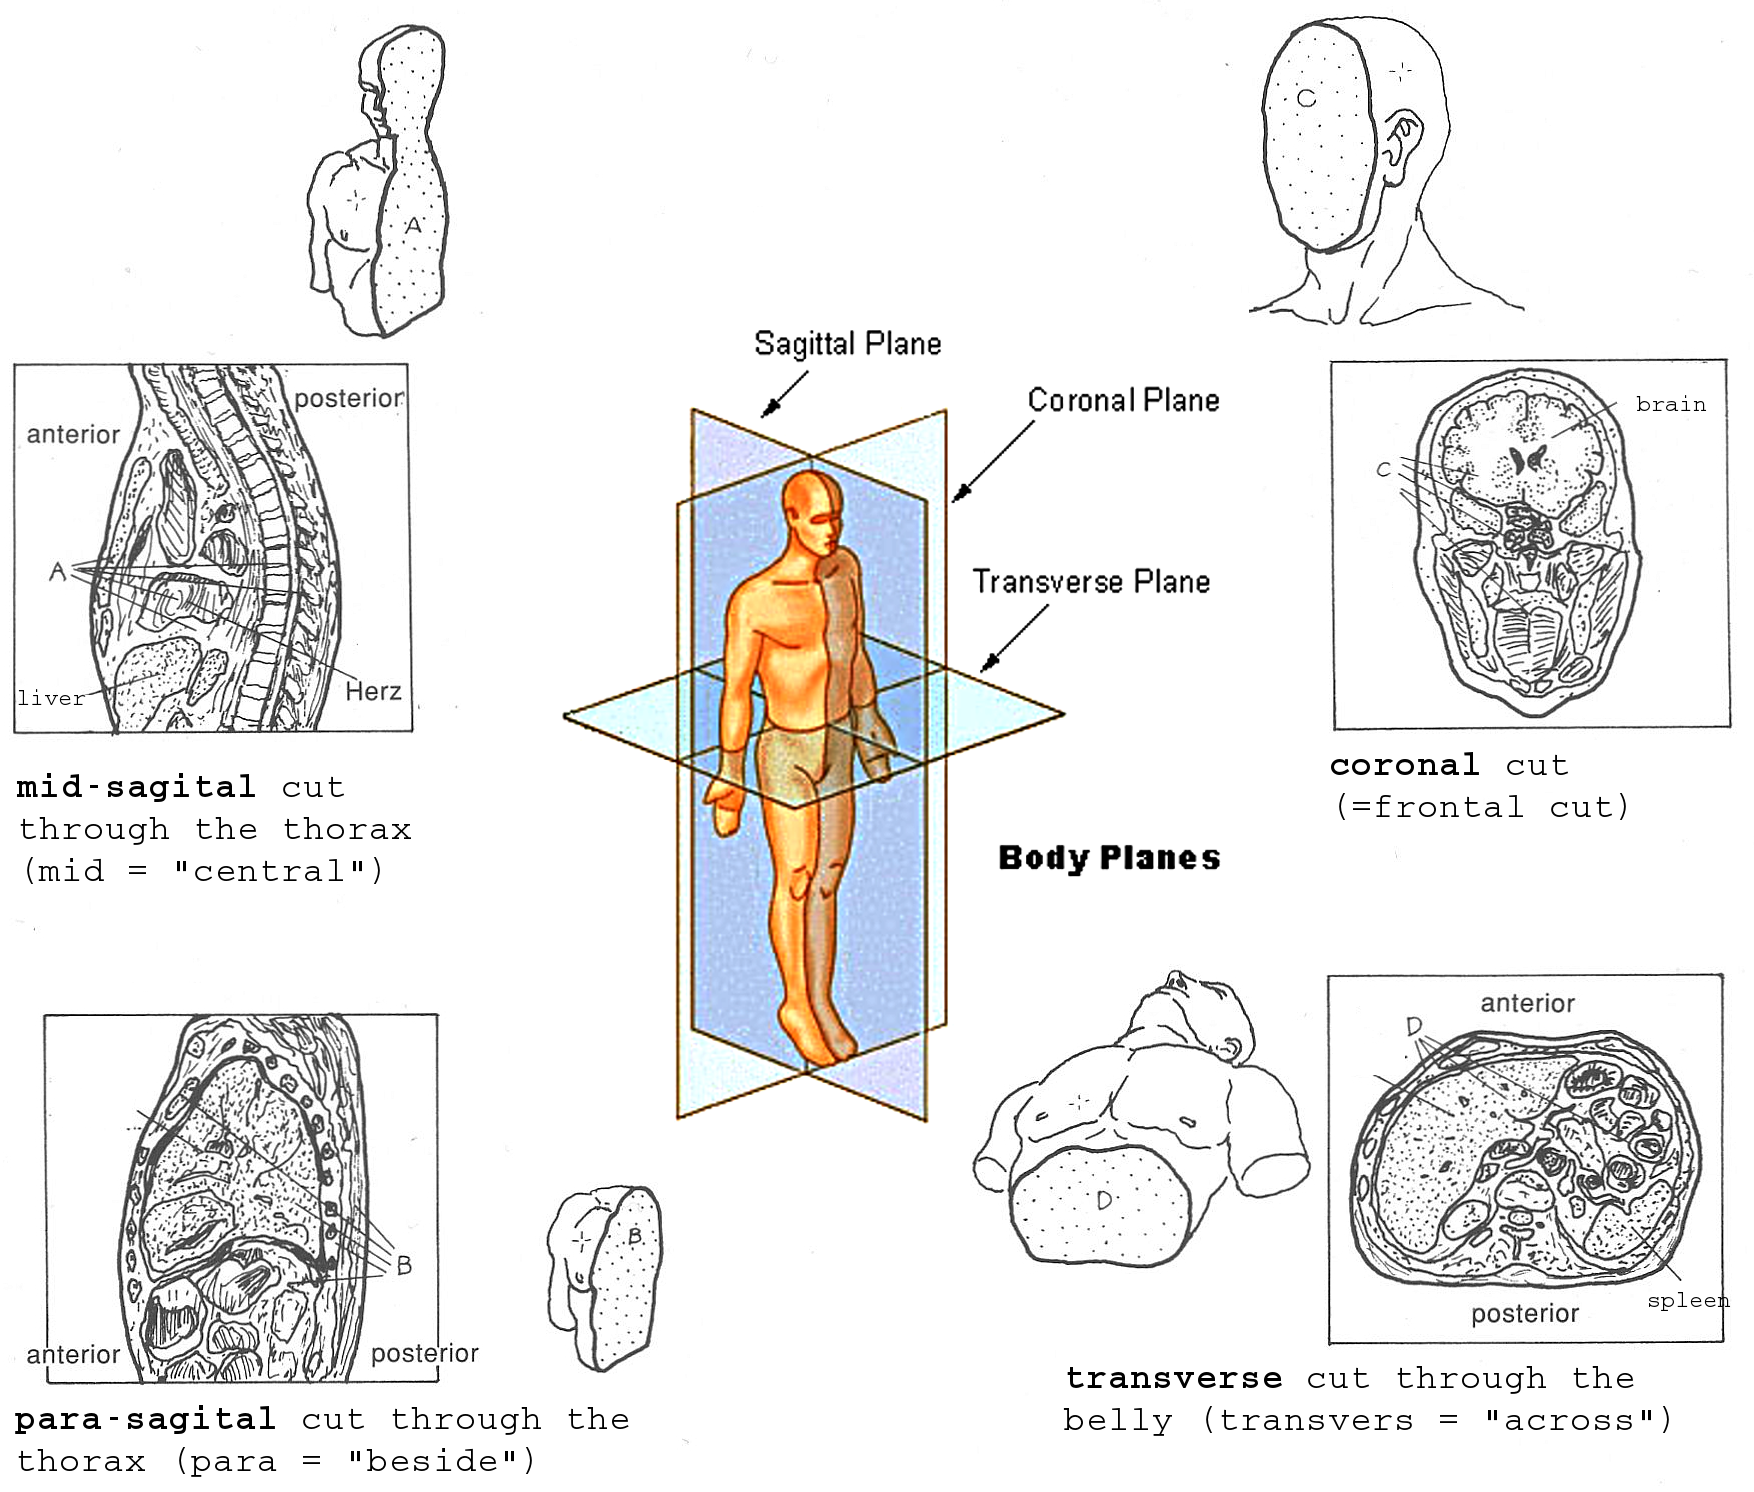
\includegraphics[width=12cm]{./Biology/hum00_anatomy/anatomical-planes-comp_v2.png}}
		\captionof{figure}[Anatomical planes AnatAtlas
		 table 1]{Anatomical planes with examples}  \label{fig:SchnittEbenen}
		\vspace{2pt}
	\end{minipage}
		
	\end{center}

		
			  \begin{figure}[htbp]
			    \begin{minipage}{0.35\textwidth}
			     \centering
			      \includegraphics[width=1\textwidth]{./Biology/hum00_anatomy/DirectionalTerms_WikiPedia_v1.png}
			      \caption{Relative anatomical terms allow to describe any point of a body relative an other point, a reference.}  \label{fig:AnatomicalTerms}
			    \end{minipage}\hspace{0.2cm}
			    \begin{minipage}{0.7\textwidth}
			     \centering
			      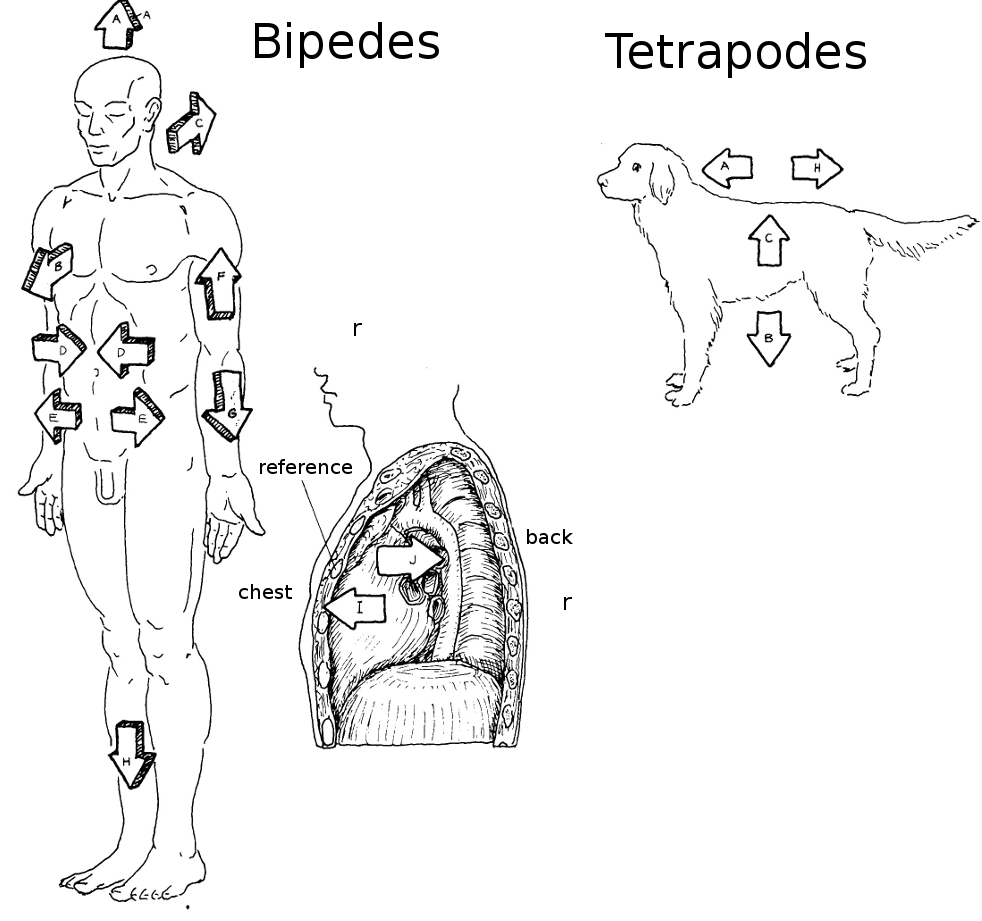
\includegraphics[width=0.9\textwidth]{/share/SB_Unterricht/Biology/hum00_anatomy/AnatomieMalatlas002_v4.png}
			      \caption{Asign the correct terms!}  \label{fig:AnatTermsApplication}
			    \end{minipage}
 				 \end{figure}
		

\areaset[0cm]{11.5cm}{26.5cm}


%  \Kommentar{visible human excluded in hs15}{}{0cm}{}
		% \subsection{A deep frozen man becomes a \emph{Visible Human}}\label{ssec:Tiefgefroren}
		% 	\begin{enumerate}[resume, leftmargin=*]
		% 	\item You are shown parts of the film
		% 			\hrefL{/share/Dropbox/Public/BlueEnd_TV-clips.avi}{}{TV-clips\textsl{``Blue End, the visible human''}} and \href{/temp/temp-filme/BlueEnd_full.avi}{Blue End, full length}
		% 		please take notes about this story. \todol{translate}
		% 		 \Loesung{
		% 	      P.J. wurde als Wiederholungstäter eingeschätzt und zum Tode verurteilt; vor der Exekution unterschrieb er, dass er einverstanden sei, der Forschung seinen Körper z.V. zu stellen; sofort nach dem Tod durch eine Giftspritze wurde P.J. Körper entwässert, tiefgefroren und alle Hohlräume mit blauem Kunststoff aufgefüllt - daher der Name des Dokumentarfilmes; der Körper wurde in mm-dicke Scheiben zerschnitten, von denen jede fotografiert und eingescannt wurde; heute stehen diese Bilder im Internet z.V.	}
		% 	      {16em}
		% 	      
		% 	\item P. J.'s body was cut in slices of 1 mm thickness. From every of these slices photos were taken and published on the world wide web. Computer animations now allow us to virtually scroll through a human body - a suspected murder became a transparent human, "` \textsl{``VisibleHuman''}. 
		% 	
		% 	Use a computer and navigate to the following website provided by the EPFL, the ETH in Lausanne:  \url{http://visiblehuman.epfl.ch/intapplet.php}. The link should take you directly to an application called  \textsc{RealTime SliceNavigation}. Be patient, the application requires quite some time to start. If the application doesn't launch and you have java enabled, you may need to apply for a login  to the website.
		% 	
		% 	\bgroup \centering \fbox{\rechts \emph{java} is required and must be allowed to run on your computer \links} \egroup
		% 	
		% 	Now take a sagital slice which runs through the chest at the height of the gall bladder. Mount here a screenshot of your slice!
		% 	
		% 	\vspace{1cm}
		% 	
		% 		    \Ersatz{
		% 				  \piccaptionoutside
		% 				  \piccaption[human longitudinal slice through the gallbladder, EPFL]{[Human longitudinal slice through the gallbladder, visible human project, EPFL}  \label{fig:bla}
		% 					\hpic[c]{\includegraphics[width=0.35\textwidth]{/share/00_SCHULE_DATA-add/bilder_saz/Humanbio_Bilder/VisibleHuman-EPFL/Liver-Gallbladder-Lungs_slice.png}}\\
		% 					The gall bladder is shown in purple; the large intestine in blue due to the blue plastic fill for all body cavities of J.P.\\
		% 					From top to bottom: lungs, liver, (right) kidney.
		% 		      }{
		% 		    \fboxsep4mm\fbox{
		% 		\begin{minipage}{8cm}
		% 			\hfill\vspace{6cm}
		% 		\end{minipage}
		% 		}}
		% 		
		% 	\end{enumerate}
		% 
		% \clearpage


\subsection{The eleven organ systems}\label{ssc:AnatOrgansysteme} 
		
		\begin{mdframed}[style=exampledefault, userdefinedwidth=12cm,frametitle={Starr 28.7}\label{mat:TenOrgansystems}]	  
			All the different tissues and organs can be grouped into eleven different systems. They are all interconnected, working together and forming together an entire system - the \textbf{body} of a human or animal.
		\end{mdframed}

	\marginnote{\caution[t][red][sickness is:]{Any disturbance in one of the eleven systems may impact all the other systems and thus sickness usually affects the entire body!}}


	\begin{enumerate}[itemsep=0.5em, leftmargin=*]   %  <ctrl-alt-i>  für "item"

		\item Enlarge the contour of the male figure shown in Fig. \ref{fig:RasterizedMale} using the enlarged grid \textit{(extra copy, A3) }!
		
		\item Add to your figure the following organs: \textsc{ heart, aorta, vena cava, lungs, diaphragm, esophagus, stomach, pancreas, small intestine, large intestine, colon, rectum, liver, gallbladder, spleen, kidneys, ureter, bladder, urethra. }\\
			(\textit{hint: you may find all these terms in  \ding{229} Starr})
		
	\end{enumerate}
			   
			   \todol{distribute A3 copies of \href{/share/SB_Unterricht/Biologie/hum00_Humanbiologie_allgemein/anat-grid_HS17.pdf}{8x4 grid} }

			   
	 	\marginnote{\caution[b][blue][The 11 organ systems]{Test yourself and list the ten organ systems by heart! (\textit{the order doesn't matter})
	 	\begin{enumerate}[label=\textit{(\arabic*)},itemsep=1em,leftmargin=1.9em,series=zaehler]
	 		\item \gap{ integumentary \hfill }
	 		\item \gap{  nervous\hfill}
	 		\item \gap{ endocrine \hfill}
	 		\item \gap{ muscular\hfill }
	 		\item \gap{ skeletal \hfill}
	 		\item \gap{ circulatory \hfill}
	 		\item \gap{ lymphatic \hfill}
	 		\item \gap{ respiratory \hfill}
	 		\item \gap{ digestive \hfill}
	 		\item \gap{ urinary \hfill}
	 		\item \gap{ reproductive \hfill}
	 	\end{enumerate}
	 	}}[12cm]
	 	

\enlargethispage{2cm}	 	

	\hspace{-1cm}
		\begin{addmargin*}[0cm]{0cm}
		 \begin{minipage}{16cm}
			\begin{overpic}[angle=0,scale=1.2,grid,tics=12.5]%
			{/share/00_SCHULE_DATA-add/bilder_saz/Humanbio_Bilder/Humanbio_Smith/smith015-2_sw_v2.jpg}
			\end{overpic}
			\vspace{2ex}  %\setcapmargin*[0cm ]{-1.5cm }  
			\captionof{figure}[Anatomie Figur aus Smith mit 8x4 Raster ]{A gride of 8 x 4 units help to learn the proportions of a human body - practise this!!}	\label{fig:RasterizedMale}
				%\setcapmargin*[0cm ]{0cm }  
		\end{minipage}
		\end{addmargin*}

	
% \vspace{\stretch{1}}
% \begin{flushright}
% \textbf{Prüfungsstoff}: Skizzieren einer menschlichen Figur in einen 4 x 8 Raster, Kenntnis der Lage der inneren Organe; einzeichnen der Organe; Kenntnis der Funktionen der 10 Organsysteme
% \end{flushright}
% 
% \clearpage
% 		\enlargethispage{4ex}	
% 			\vspace{4pt}
% 		
% 			 \begin{center}
% 				\begin{minipage}[htbp]{1\columnwidth}
% 			 \centering
% 				\begin{tikzpicture}[scale=2.9]
% 					\draw (0,0) grid (4,8);
% 				\end{tikzpicture}
% 					\captionof{figure}[8x4 Raster tzkip-pict]{Grid to draw an anatomical figure - see figure \ref{fig:RasterFiguren}}  \label{fig:AnatRaster}
% 				\end{minipage}
% 			   \end{center}

% \areaset[0cm]{11.5cm}{26.5cm}  


